\chapter{Análisis y experimentación}
\label{chap:analisis-y-experimentacion}

Una vez adquiridos los conocimientos teóricos necesarios, y comprendido el funcionamiento de los diferentes algoritmos que vamos a utilizar, estamos en disposición de aplicarlos a los datos de experimentación y comprobar la eficacia de los algoritmos en un caso real. Este capítulo aborda el trabajo realizado durante tres meses en el Instituto Cajal, aplicando diferentes técnicas para tratar de agrupar los comportamientos de los animales, y de diferenciar animales bajo efectos de tratamiento o de placebo.

En la Sección \ref{sec:preprocesado} tratamos como hemos preprocesado los videos para homogeneizar todas las sesiones de experimentación, obtener los datos de posición de los animales en ellas y filtrar e interpolar los datos poco verosímiles. En la Sección \ref{sec:análisis} desarrollamos el proceso de análisis de los datos preprocesados aplicando los diferentes algoritmos vistos anteriormente y analizando sus resultados.

\section{Preprocesado de datos} \label{sec:preprocesado}

Los datos de los que hemos partido para realizar el análisis han sido 88 pares de videos en blanco y negro, de unos cinco minutos cada uno, de ratones en su caja sin estar realizando ninguna tarea concreta. Cada par de videos consistía en un video de la vista cenital de la caja y otro de la vista lateral, como se puede observar en la Figura \ref{fig:deeplabcut-outputexamples}. Además, de cada par de videos teníamos el código del animal que estaba siendo grabado, la fecha de la sesión y si el animal estaba bajo los efectos del tratamiento de NDMA en dicha fecha o no. Mostramos un resumen de estos datos en la Tabla \ref{tab:animal-info}.

% Animal info
\begin{table}[h]
  \centering
  \begin{tabular}{|c|c|c|c|}
    \hline
    \textbf{Video} & \textbf{Código del animal} & \textbf{Fecha de la sesión} & \textbf{Tratamiento} \\ 
    \hline
    1 & 4128	& 2020-12-02	& CONTROL \\ 	
    2 & 4128	& 2020-11-21	& CONTROL \\ 	
    3 & 4128	& 2020-11-23	& CONTROL \\ 
    ... &  ...	& ... & ... \\ 
    80 & 4108	& 2020-09-25	& NMDA	\\ 
    81 & 4089	& 2020-09-18	& NMDA	\\
    82 & 4089	& 2020-09-12	& CONTROL	\\ 
    83 & 4089	& 2020-09-24	& NMDA	\\
    \hline
  \end{tabular}
  \caption[Datos de las sesiones]{Fragmento del \texttt{DataFrame} que almacenaba los datos de las sesiones, incluyendo el número del video según se almacenaban en memoria, el código del animal, la fecha de la sesión y el estado del tratamiento.}
  \label{tab:animal-info}
\end{table}

Para tratar de averiguar de forma automática el tipo de tratamiento de cada sesión, podríamos entrenar una red neuronal utilizando directamente los videos como datos de entrenamiento. Sin embargo, no contamos con una cantidad muy elevada de videos para entrenar, y además esto no nos daría ninguna pista sobre como comportamientos concretos se relacionan con el tratamiento. Al no contar con una base de datos de fragmentos de videos clasificados según el comportamiento del animal, tampoco podemos entrenar una red para distinguir estos comportamientos sin tener que pasar antes por un seguramente tedioso periodo de etiquetado manual de fragmentos. Por ello, hemos hecho uso de la herramienta DeepLabCut para rastrear la posición del ratón en cada fotograma y así poder hacer cálculos sobre ella, y trabajar con otros algoritmos de agrupación no supervisada para tratar de clasificar diferentes movimientos del ratón a lo largo del video.

\subsection{DeepLabCut}\label{sec:DeepLabCut}

(EXPLICACIÓN DEEPLABCUT)

% DeepLabCut output
\begin{figure}[p]
  \centering
  \begin{subfigure}{0.45\textwidth}
    \centering
    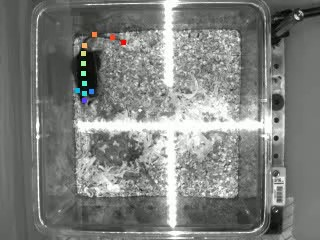
\includegraphics[width=\textwidth, angle=-90]{figures/deeplabcut-top-example-4128-2020-12-02-1-00-37.jpg}
    \caption{}
    \label{fig:deeplabcut-top-example}
  \end{subfigure}
  \begin{subfigure}{0.45\textwidth}
    \centering
    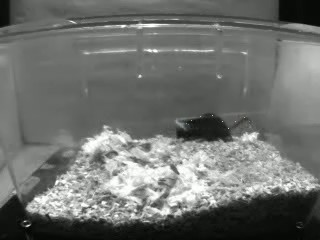
\includegraphics[width=\textwidth]{figures/deeplabcut-lateral-example-4128-2020-12-02-1-00-37.jpg}
    \caption{}
    \label{fig:deeplabcut-lateral-example}
  \end{subfigure}
  \begin{subfigure}{0.45\textwidth}
    \centering
    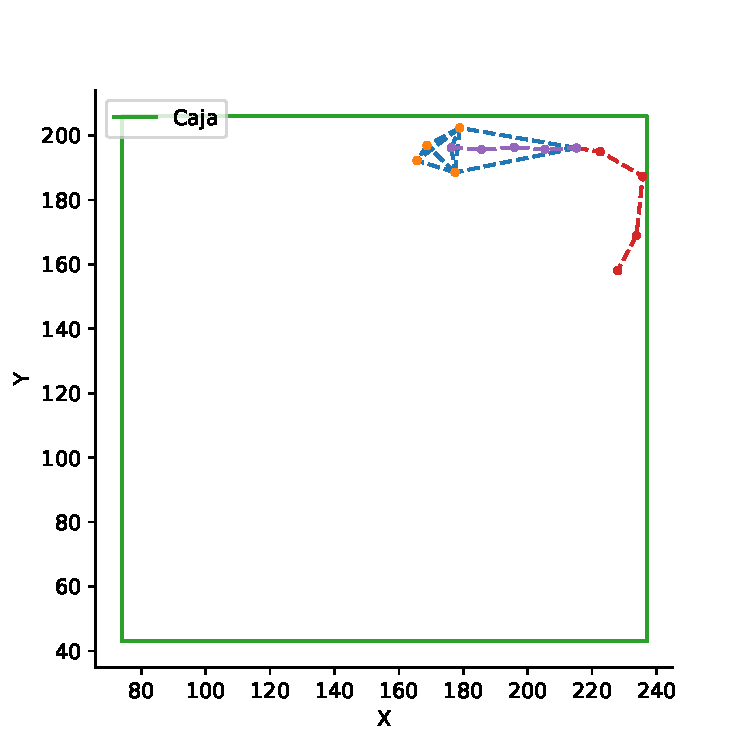
\includegraphics[width=\textwidth]{figures/triangulation-top-4128-2020-12-02.pdf}
    \caption{}
    \label{fig:triangulation-top}
  \end{subfigure}
  \begin{subfigure}{0.45\textwidth}
    \centering
    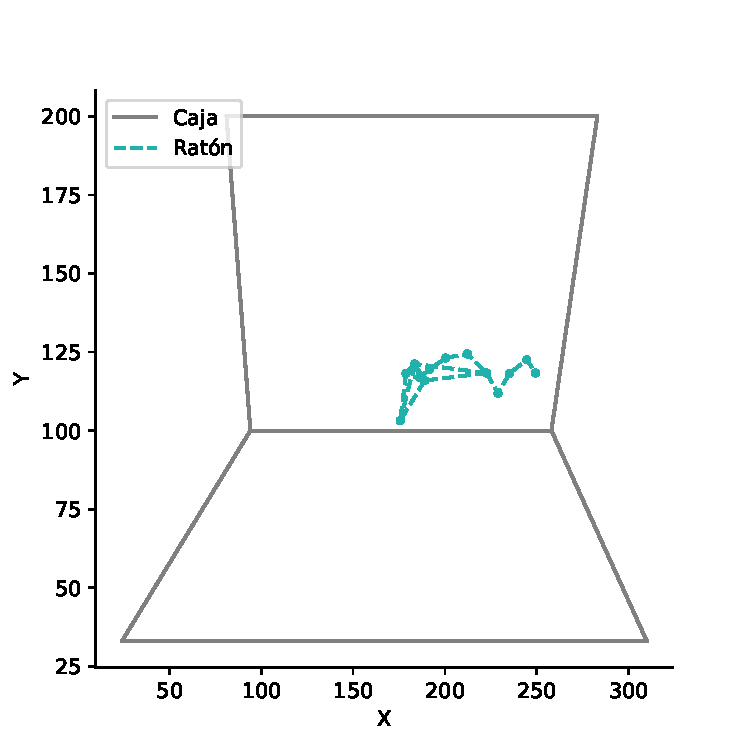
\includegraphics[width=\textwidth]{figures/triangulation-lateral-4128-2020-12-02.pdf}
    \caption{}
    \label{fig:triangulation-lateral}
  \end{subfigure}
  \caption[Salida de DeepLabCut.]
  {Salida de DeepLabCut del animal 4128 el 02-12-2020, 1:00:37. \ref{fig:deeplabcut-top-example} Video de la vista cenital de la caja. Los puntos sobre el animal son los dibujados por DeepLabCut para rastrear las partes del animal. \ref{fig:deeplabcut-lateral-example} Video de la vista lateral de la caja. \ref{fig:triangulation-top} En azul, la triangulación formada por los puntos obtenidos por DeepLabCut de la vista cenital. Cinco puntos para la cabeza, cuatro para la espalda y otros cuatro para la cola. En gris, las dimensiones de la base de la caja, obtenidas midiendo las distancias en píxeles sobre un fotograma de video. \ref{fig:triangulation-lateral} Análogo a la vista cenital, desde la vista lateral. En gris, la altura mínima del suelo de la caja y su pared trasera.}

  \label{fig:deeplabcut-outputexamples}
\end{figure}

% Dataframe example
\begin{table}[h]
  \centering
  \begin{tabular}{|c|c|c|c|c|c|c|}
  \hline
    & Nosex & Nosey & Noselikelihood & Headx & Heady & ... \\
  \hline
  0 & 136.165344 & 177.722496 & 0.000084 & 129.790253 & 174.772552 & ... \\
  1 & 162.032005 & 201.444756 & 0.942181 & 168.152061 & 202.420639 & ... \\
  2 & 156.297043 & 200.326378 & 0.000073 & 162.436028 & 203.156837 & ... \\
  3 & 155.370415 & 199.043297 & 0.000277 & 159.507599 & 200.199928 & ... \\
  4 & 149.272644 & 197.677170 & 0.000045 & 155.493912 & 198.814835 & ... \\
  ... & ... & ... & ... & ... & ... & ... \\
  \hline
  \end{tabular}
  \caption[Datos de DeepLabCut]{Extracto del \texttt{DataFrame} de \texttt{pandas} de los datos sin procesar de DeepLabCut. Para cada punto rastreado, y para cada fotograma del video, se computa la predicción de la coordenada $x$ y de la coordenada $y$ y se da la verosimilitud de dicha predicción.}
  \label{tab:df-example}
\end{table}

\subsection{Filtrado e interpolación}
Una vez hemos pasado todos los videos por DeepLabCut, tenemos dos ficheros de datos para cada uno de las sesiones, uno para las coordenadas de los puntos de la vista cenital y otro para las coordenadas de los puntos de la vista lateral. Al cargar los ficheros a memoria como \texttt{DataFrames} de \texttt{pandas}, vemos que no todos ellos tienen la misma duración, por lo que los homogeneizamos todos eliminando los datos de los últimos fotogramas, consiguiendo que cada \texttt{DataFrame} tenga un tamaño de 6000 filas, lo que equivale a 6000 fotogramas o 5 minutos de video. Además, eliminamos los datos de 4 videos que no llegan a esa duración, ya que son videos con problemas que entorpecerían el análisis. Finalmente, eliminamos los datos de 2 videos más, ya que tras el preprocesado seguían teniendo valores nulos debido a que DeepLabCut no ha podido identificar varios de los puntos a rastrear en ninguno de los fotogramas de los videos.


% Trayectory prerpocessing
\begin{figure}[p]
  \centering
  \begin{subfigure}{0.38\textwidth}
    \centering
    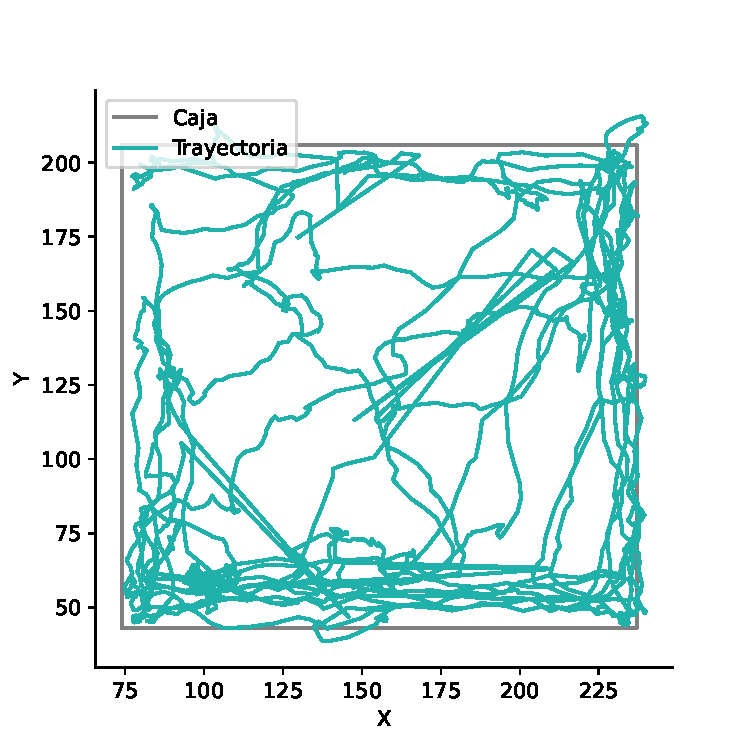
\includegraphics[width=\textwidth]{figures/raw-trayectory-top-4128-2020-12-02.pdf}
    \caption{}
    \label{fig:raw-top}
  \end{subfigure}
  \begin{subfigure}{0.38\textwidth}
    \centering
    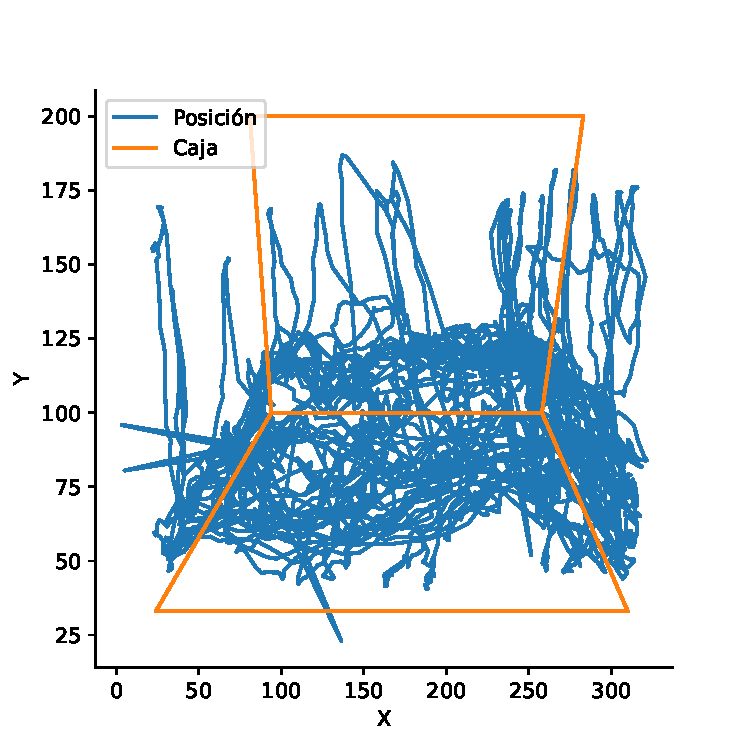
\includegraphics[width=\textwidth]{figures/raw-trayectory-lateral-4128-2020-12-02.pdf}
    \caption{}
    \label{fig:raw-lat}
  \end{subfigure}
  \begin{subfigure}{0.38\textwidth}
    \centering
    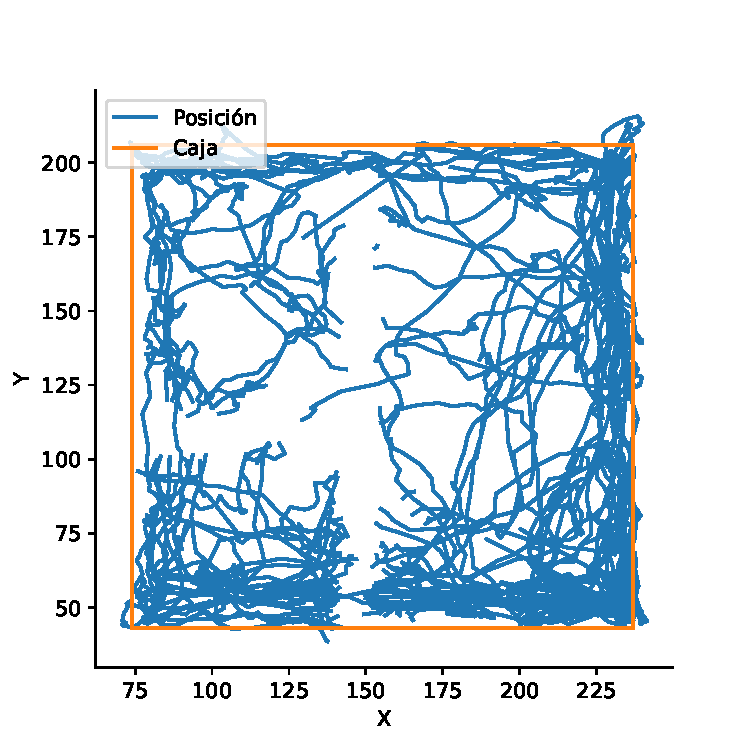
\includegraphics[width=\textwidth]{figures/filtered-trayectory-top-4128-2020-12-02.pdf}
    \caption{}
    \label{fig:filter-top}
  \end{subfigure}
  \begin{subfigure}{0.38\textwidth}
    \centering
    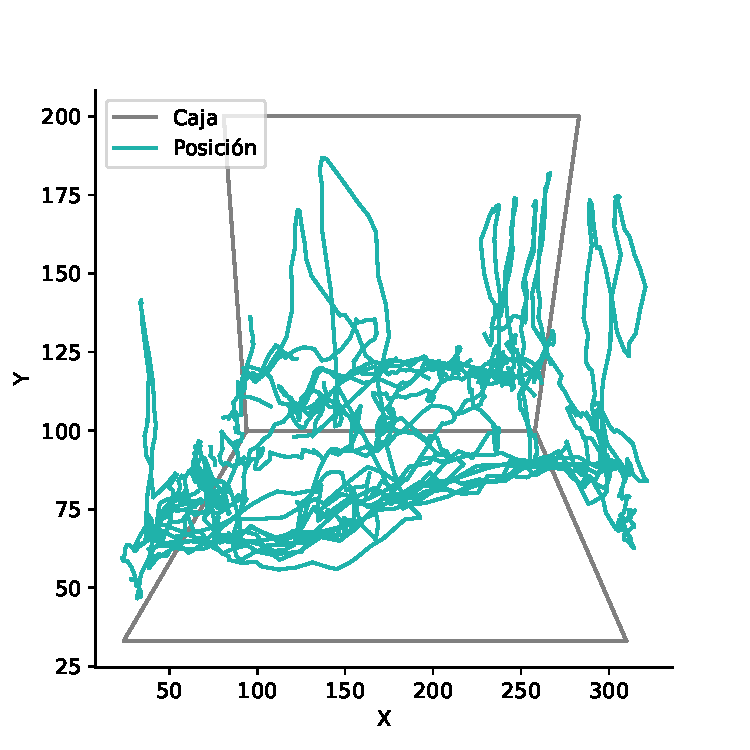
\includegraphics[width=\textwidth]{figures/filtered-trayectory-lateral-4128-2020-12-02.pdf}
    \caption{}
    \label{fig:filter-lat}
  \end{subfigure}
  \begin{subfigure}{0.38\textwidth}
    \centering
    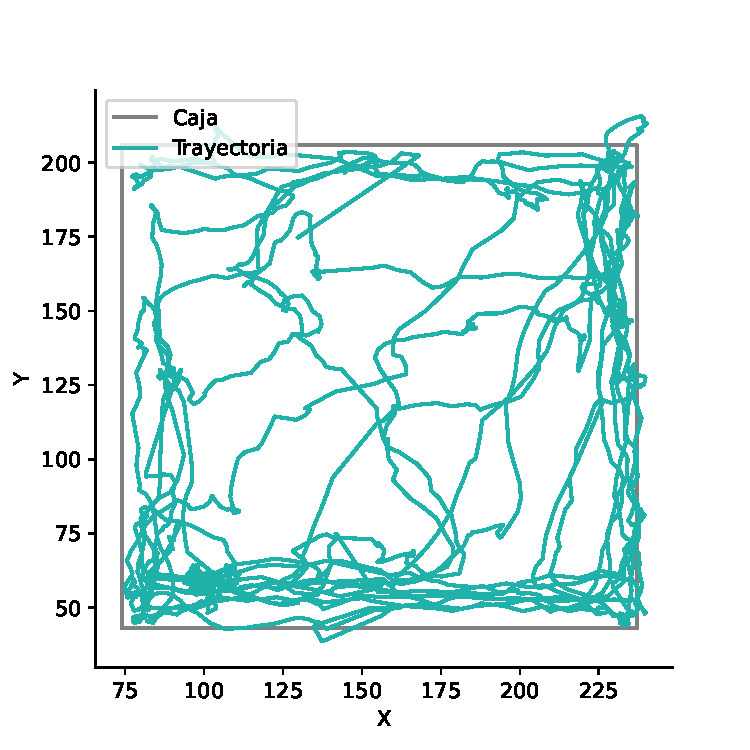
\includegraphics[width=\textwidth]{figures/interpolated-trayectory-top-4128-2020-12-02.pdf}
    \caption{}
    \label{fig:inter-top}
  \end{subfigure}
  \begin{subfigure}{0.38\textwidth}
    \centering
    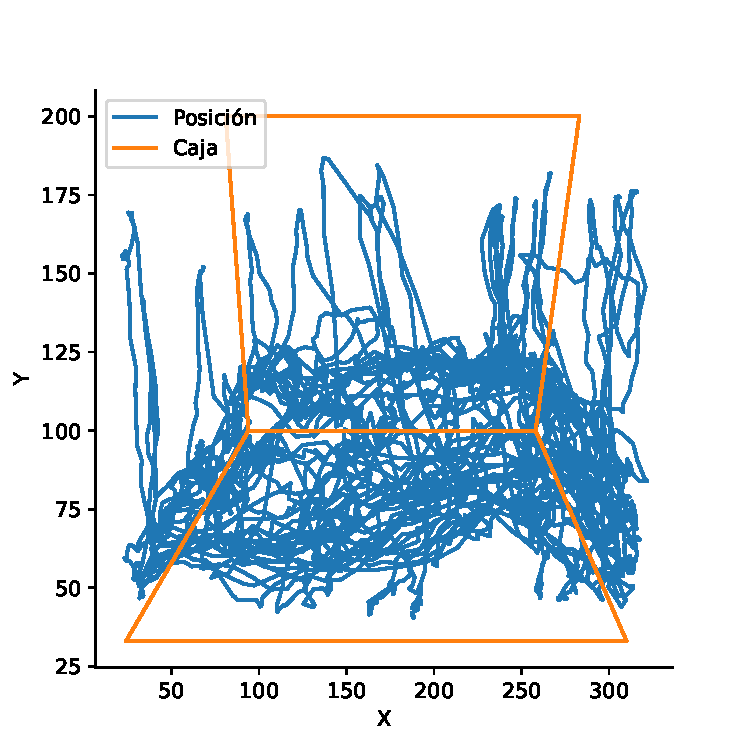
\includegraphics[width=\textwidth]{figures/interpolated-trayectory-lateral-4128-2020-12-02.pdf}
    \caption{}
    \label{fig:inter-lat}
  \end{subfigure}
  \caption[Trayectorias durante el preprocesamiento.]{Vistas cenital y lateral de trayectorias de un punto de la cabeza del animal 4128. Datos correspondientes a los dos primeros minutos de la sesión del 2020-12-02. \ref{fig:raw-top}, \ref{fig:raw-lat}: Vista cenital de los datos antes del preprocesado. En gris se ha dibujado las dimensiones de la caja y en color la trayectoria del punto \texttt{Head}. \ref{fig:inter-top}, \ref{fig:inter-lat}: Vistas cenital y lateral de los datos una vez filtrados los valores de baja berosimilitud. \ref{fig:inter-top}, \ref{fig:inter-lat}: Vistas cenital y lateral de los datos filtrados con los valores nulos interpolados. }
  \label{fig:interpolated-trayectories}
\end{figure}


%\subsection{Computo de variables a analizar}

%Una vez todos los datos han sido preprocessados, podemos computar diferentes propiedades de los mismos para usarlas posteriormente en los algoritmos de agrupación o de reducción de dimensiones. Además, podemos computar puntos de mayor confianza calculando medias de otros puntos individuales.

%(FINALIZAR SECCIÓN e INCLUIR FIGURAS)

\newpage
\section{Análisis de datos} \label{sec:análisis}

\subsection{Clasificación manual de comportamientos.}
Gracias a los datos de DeepLabCut podemos tratar de identificar ciertos comportamientos de forma manual, especificando ciertos umbrales para extraer los comportamientos deseados. A modo de ejemplo, hemos calculado cuando el punto de la cabeza en la vista cenital, \texttt{head}, se salía durante un intervalo de cinco fotogramas fuera de los límites establecidos de la caja. Así, como se observa en la Figura \ref{fig:rearing}, hemos identificado los intervalos de tiempo de cada sesión en los cuales el animal se alza sobre sus extremidades traseras apoyándose en la pared de la caja.

% Rearing frames
\begin{figure}[h]
  \centering
  \begin{subfigure}{\textwidth}
    \centering
    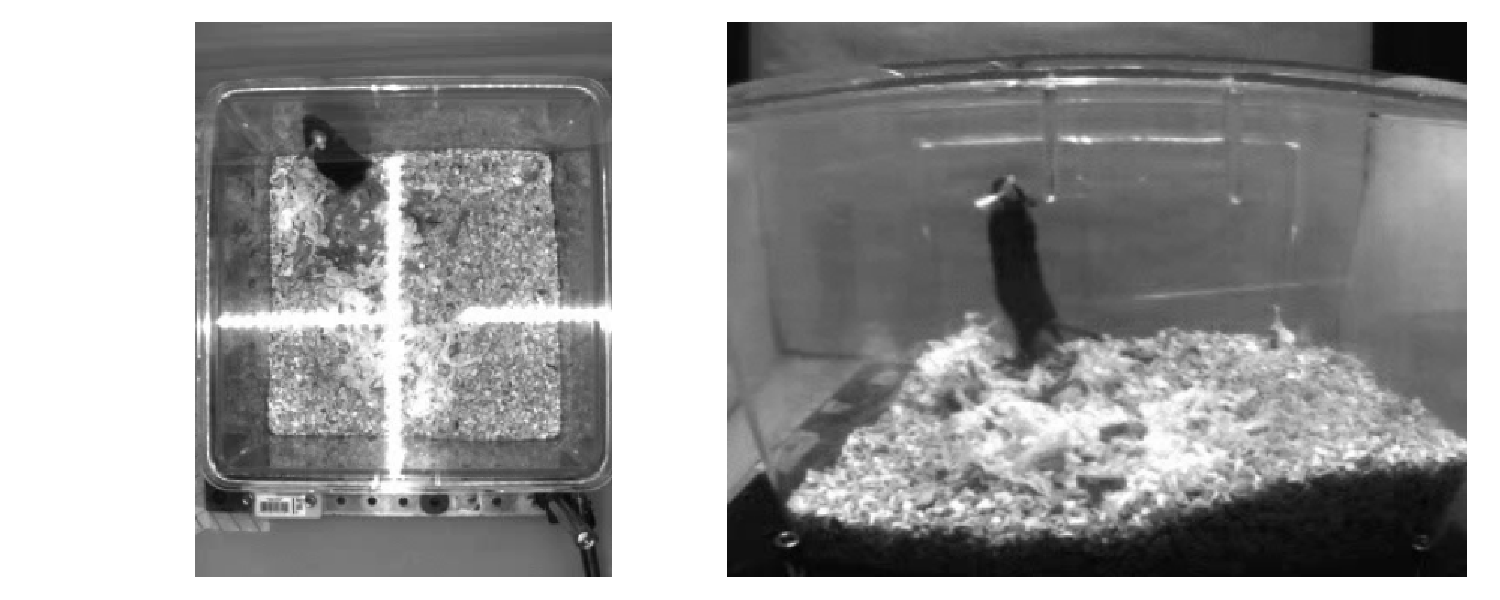
\includegraphics[trim={2cm 0 0 0}, width=0.9\textwidth]{figures/rearing-4128-2020-12-02-0 03.05.pdf}
  \end{subfigure}
  \begin{subfigure}{\textwidth}
    \centering
    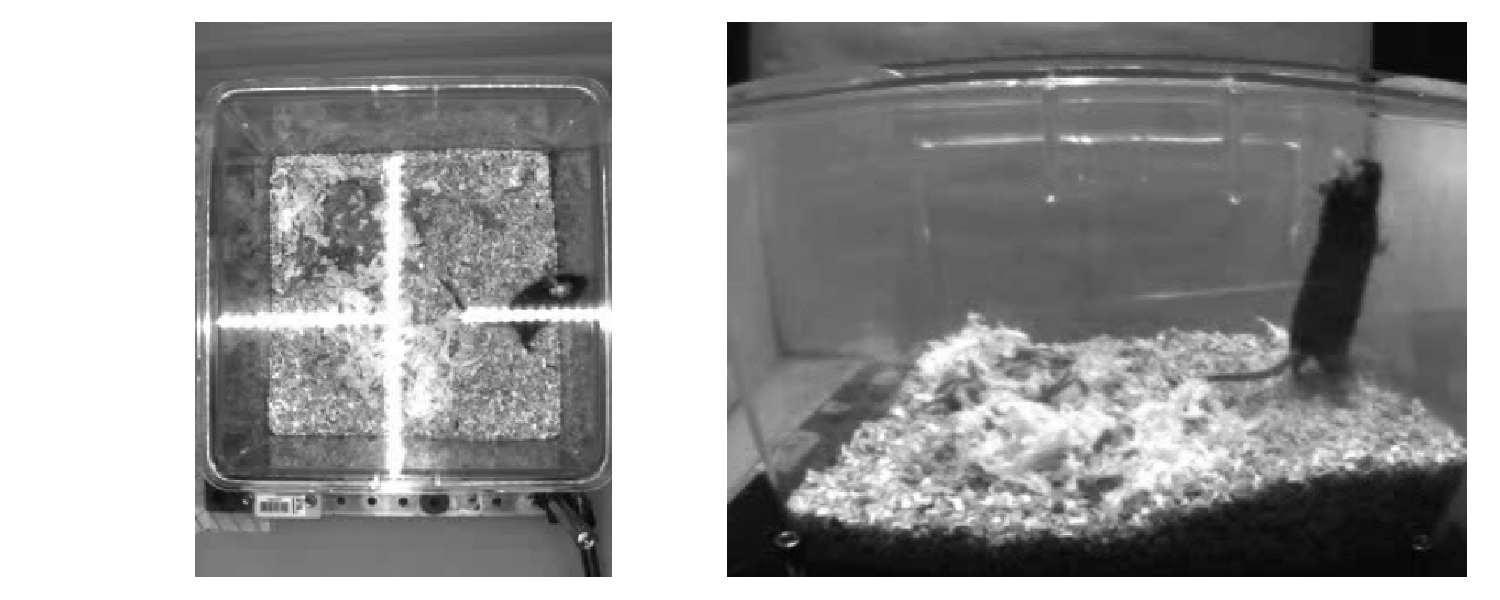
\includegraphics[trim={2cm 0 0 0}, width=0.9\textwidth]{figures/rearing-4128-2020-12-02-0 19.43.pdf}
  \end{subfigure}
  \caption[Fotogramas del animal alzándose.]{Fotogramas de los dos primeros intervalos en los que el animal 4128 se alza en la sesión del 2020-12-02. Los fotogramas superiores corresponden a la vista cenital y lateral del segundo 3,05. Los fotogramas inferiores corresponden a las mismas vistas del segundo 19,43.}
  \label{fig:rearing}
\end{figure}

De la misma forma, podemos calcular en que intervalos la media de los puntos de la espalda tienen una velocidad mayor de tres píxeles por segundo para identificar cuando el animal se está moviendo como se puede ver en la Figura \ref{fig:speed}, o calcular el ángulo formado entre un vector de los puntos de la cabeza del animal y otro de los puntos de la espalda, para determinar si el animal está girado hacia algún lado, visualizado en la Figura \ref{fig:angles}.

% Speed
\begin{figure}[h]
  \centering
  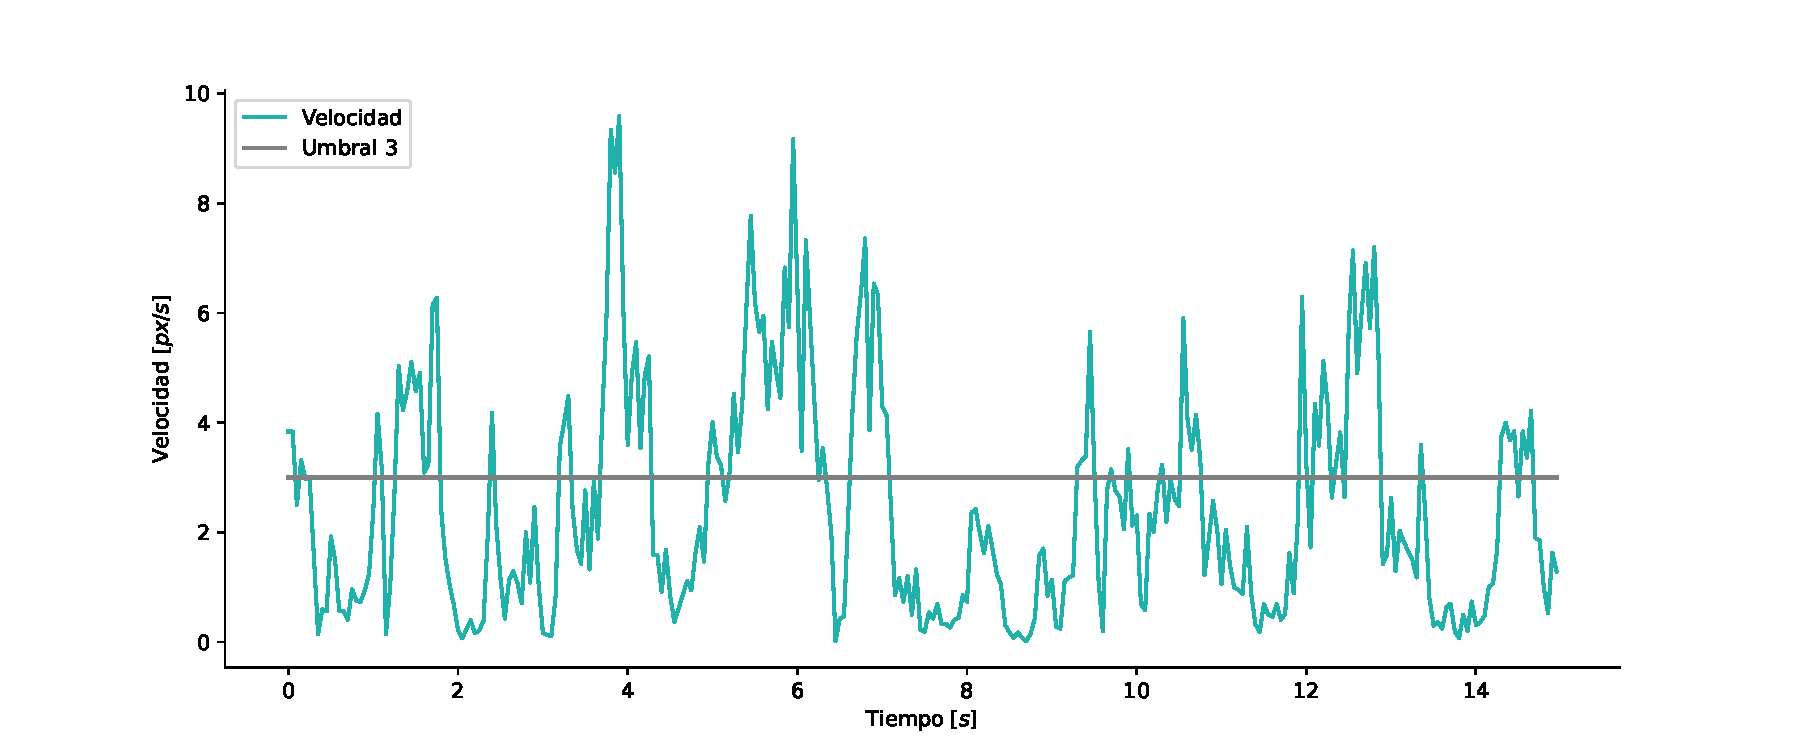
\includegraphics[width=\textwidth]{figures/speed-4128-2020-12-02-threshold-3-15s.pdf}
  \caption[Velocidad del animal.]{Gráfico de la velocidad del animal 4128, durante los primeros 15 segundos de la sesión del 2020-12-02. En color, los datos obtenidos derivando la trayectoria de la media de los puntos de la espalda del animal: \texttt{Neck}, \texttt{Back\_1}, \texttt{Back\_2}, \texttt{Back\_3} y \texttt{Back\_4}. En gris, el umbral arbitrario de 3 píxeles por segundo, para diferenciar cuando el animal está desplazándose y cuando no.}
  \label{fig:speed}
\end{figure}

% Angles
\begin{figure}[h]
  \centering
  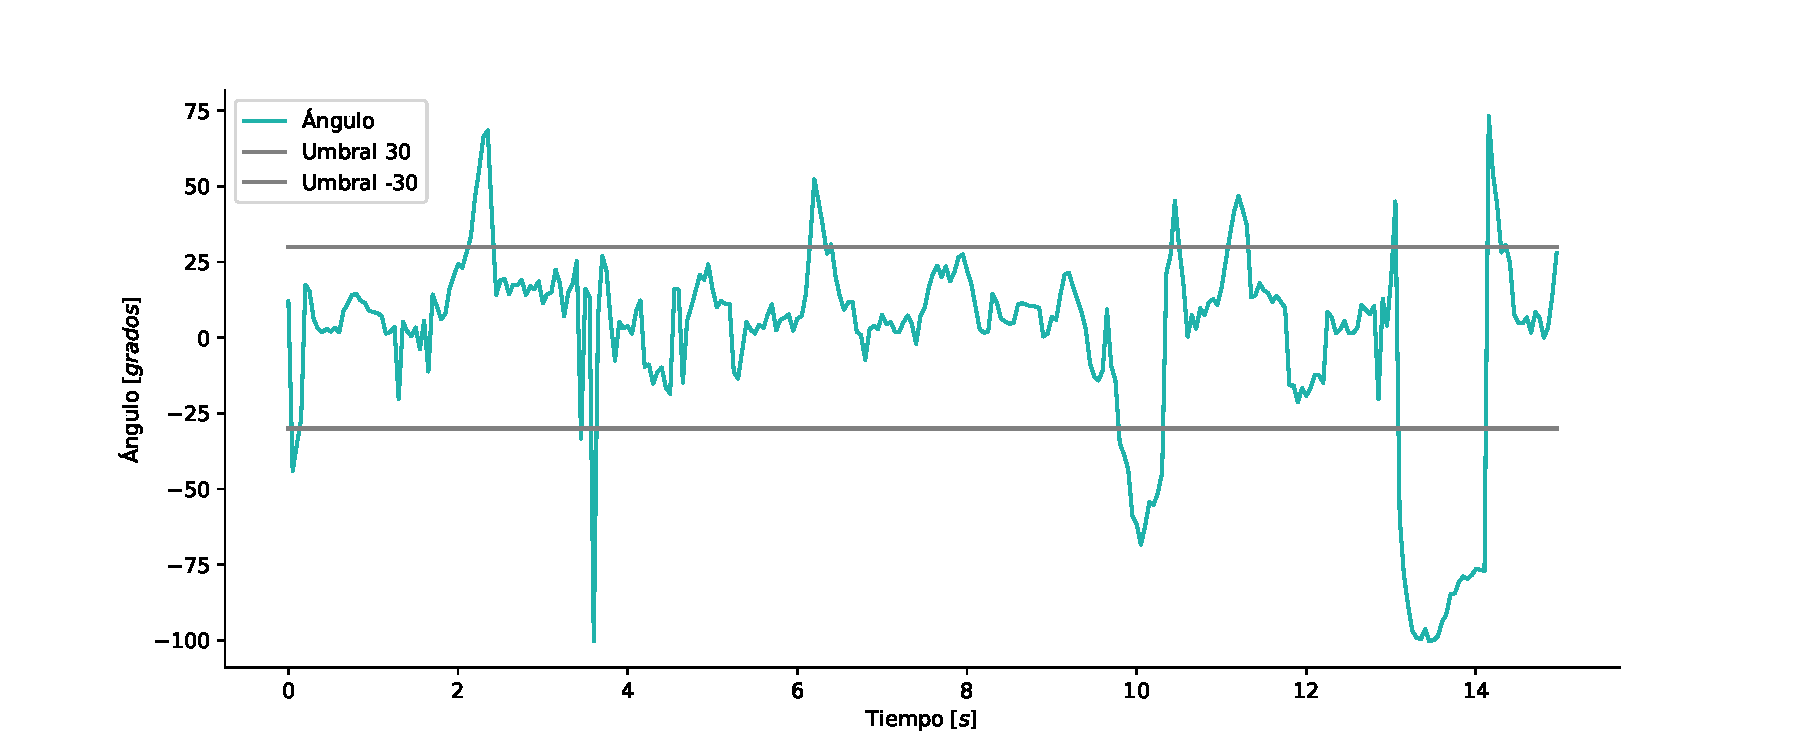
\includegraphics[width=\textwidth]{figures/angles-4128-2020-12-02-threshold-30-15s.pdf}
  \caption[Ángulos del animal.]{Gráfico de los ángulos del animal 4128, durante los primeros 15 segundos de la sesión del 2020-12-02. En color, el ángulo formado por el vector de los puntos de la cabeza con el vector de los puntos de la espalda. En gris, los umbrales de 30° y -30° para determinar si el animal está recto, o tiene el cuerpo girado hacia la izquierda o derecha respectivamente,}
  \label{fig:angles}
\end{figure}

Estos métodos de extracción de comportamientos funcionan para este caso particular, pero al depender de funciones hechas específicamente para estos datos, sería complejo exportarlo a otros escenarios. DeepLabCut ayuda en ese aspecto, ya que no calculamos propiedades sobre los videos en sí, sino sobre un conjunto de coordenadas de posiciones de partes del animal. De esta forma, si se tratase de analizar videos de animales grabados en otras cajas o realizando alguna tarea, podríamos computar de forma sencilla estas propiedades ajustando los parámetros necesarios.

Sin embargo, para el cómputo manual de estas propiedades se han puesto umbrales arbitrarios para definir el estado del animal. Un umbral de 3 píxeles por segundo sobre la media de los puntos de la espalda para determinar cuando el animal se está desplazando, un umbral de ±30° para determinar si el animal está girando o no, o un umbral de 5 fotogramas fuera de las dimensiones de la caja para determinar si el animal se está alzando sobre una pared. Los umbrales son necesarios si consideramos necesario discretizar estas variables continuas en comportamientos cualitativos, pero están a su vez sesgados por el juicio del experimentador, ya que una varianza en la magnitud de los umbrales o en el conjunto de puntos utilizados para calcularlos puede resultar en una discrepancia de la clasificación obtenida.

La clasificación manual hace que sea complejo determinar también cuando el animal realiza algún comportamiento más complejo que los vistos hasta ahora, ya que si no sabemos de antemano la relación entre las coordenadas de las partes del animal y el comportamiento, no podremos identificarlo. De la misma forma, al no conocer de antemano la relación entre los diferentes comportamientos y el tipo de tratamiento dado a los animales, con estas clasificaciones no se podrán diferenciar animales tratados con anticuerpos de NDMA de animales control.

Esto motiva las siguientes secciones en las cuales hemos utilizado diversos métodos de aprendizaje automático para tratar de conseguir clasificaciones sin depender de sesgos preestablecidos.

\subsection{Agrupaciones no supervisadas.}
Para tratar de automatizar el proceso de clasificación, sin depender de cualidades computadas \textit{ad hoc} para este conjunto de datos, hemos realizado los algoritmos vistos en la sección \ref{sec:unsupervised} sobre los datos de las trayectorias preprocesados según hemos visto en la sección \ref{sec:preprocesado}.

Para clasificar los comportamientos de un animal en cada sesión no contamos con datos previamente clasificados por lo que no podemos hacer uso de métodos de aprendizaje automático supervisados. Además, si no queremos introducir un sesgo en la clasificación, tampoco sabemos de antemano en cuantos grupos de comportamiento similares podremos agrupar los diferentes fragmentos de cada sesión de video. Por ello hemos utilizado un algoritmo de propagación de afinidad, basándonos en el trabajo realizado en \cite{neuron}, con el cual podemos realizar una agrupación de intervalos de tiempo en función de su afinidad. Pese a todo ello, hay que introducir un pequeño sesgo en el proceso, determinando arbitrariamente la longitud de los intervalos de tiempo que queremos clasificar. Hemos dividido los videos de las sesiones en intervalos de 5 segundos e introducido los datos de las coordenadas de todos los puntos de las vistas cenital y lateral para todos los puntos de cada fotograma de los intervalos. En la Figura \ref{fig:unsupervied-behav} se muestra la agrupación obtenida para la sesión de uno de los animales, consiguiendo agrupar los distintos intervalos en 7 grupos de comportamiento.

% Behav aff
\begin{figure}[h]
  \centering
  \begin{subfigure}{0.45\textwidth}
    \centering
    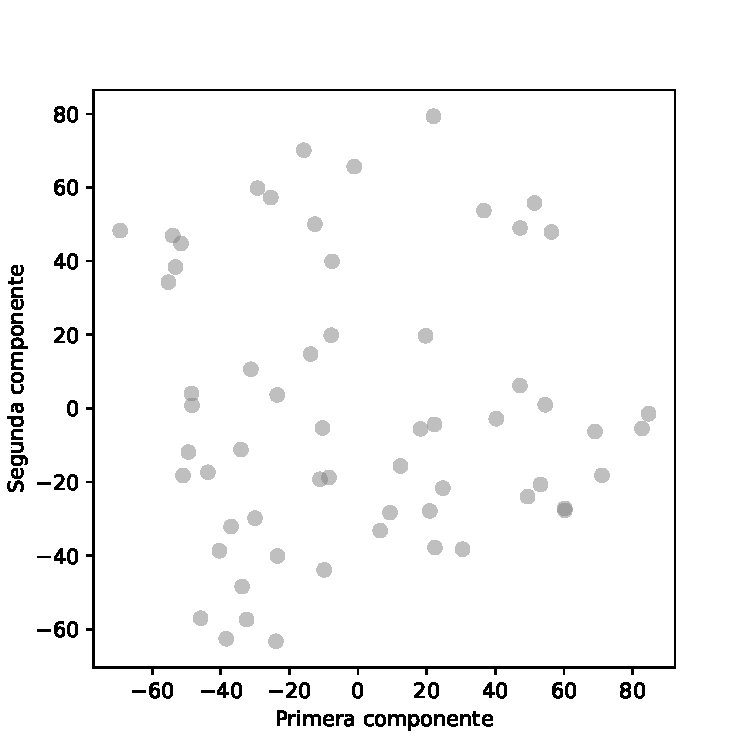
\includegraphics[width=\textwidth]{figures/behav-pca-4128-202012-02.pdf}
    \caption{}
    \label{fig:behav-pca}
  \end{subfigure}
  \begin{subfigure}{0.45\textwidth}
    \centering
    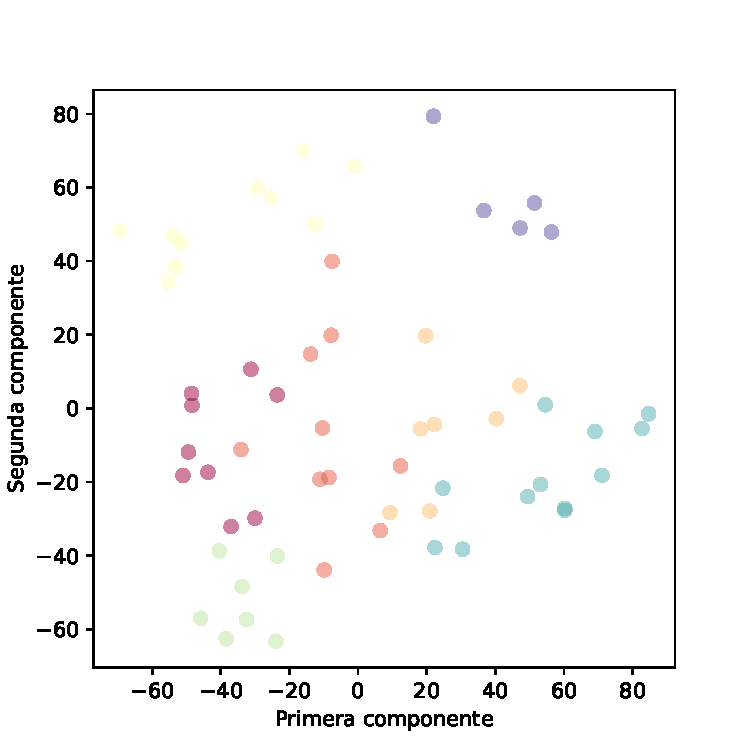
\includegraphics[width=\textwidth]{figures/behav-aff-4128-202012-02.pdf}
    \caption{}
    \label{fig:behav-aff}
  \end{subfigure}
  \caption[Clasificación no supervisada de comportamiento.]{Clasificación de comportamiento mediante el algoritmo de propagación de afinidad sobre intervalos de la sesión del animal 4128 el 2020-12-02. \ref{fig:behav-pca}: Distribución de los puntos de un PCA sobre una subdivisión de la sesión en 60 intervalos. Cada punto representa un intervalo de 5 segundos, 100 fotogramas, de la sesión de video. Cada punto original cuenta con 56 dimensiones, correspondientes a las coordenadas $ x $ e $ y $ de los 14 puntos extraídos por DeepLabCut tanto para la vista cenital como la vista lateral. Todos los puntos se han normalizado para tener media 0 y desviación 1 antes de realizar el PCA. Tras el PCA, y únicamente para su representación gráfica, se conservan las dos primeras componentes principales de cada punto. \ref{fig:behav-aff}: Misma representación de los 60 intervalos que en \ref{fig:behav-pca}, pero los puntos han sido coloreados según el número de grupo asignado por el algoritmo de propagación de afinidad. El algoritmo se ha realizado sobre los puntos de los intervalos normalizados, manteniendo las 56 dimensiones originales y utilizando la norma euclídea como medida de afinidad.}
  \label{fig:unsupervied-behav}
\end{figure}

Para diferenciar el tipo de tratamiento de cada una de las sesiones utilizando los datos de DeepLabCut mediante algoritmos no supervisados, no podemos usar el algoritmo de propagación de afinidad, ya que no es posible garantizar que vaya a generar dos únicas clases. Por ello, hemos utilizado los otros dos algoritmos explicados en la sección \ref{sec:unsupervised}: la agrupación por k-medias y la agrupación aglomerativa, ambos utilizados en estudios similares \cite{frontiers}. Para ambos casos hemos tomado los datos de todas las sesiones y tras aplicarles el algoritmo hemos mostrado los resultados en la Figura \ref{fig:unsupervied-treatment}. Con ninguno de los dos algoritmos hemos conseguido resultados significativamente mejores que los que obtendríamos haciendo asignaciones aleatorias de las clases, con lo que podemos asumir que no hay ninguna relación directa entre la posición de los animales y el tipo de tratamiento que se les ha suministrado.

Para conseguir realizar esta clasificación habría que computar otras características manualmente con las que dar más información a los algoritmos, cambiar los puntos rastreados por DeepCutLab para conseguir información sobre otras partes del animal, o tratar de predecir una función desconocida que fuera capaz de agrupar las sesiones correctamente. Como tenemos los datos de todas las sesiones podemos entrenar métodos supervisados, y estamos en las condiciones idóneas para tratar de predecir, en caso de que exista, esa función que relacione las coordenadas de los puntos que hemos rastreado con el tipo de tratamiento de cada sesión.

% Treatment kmean agg
\begin{figure}[p]
  \centering
  \begin{subfigure}{0.45\textwidth}
    \centering
    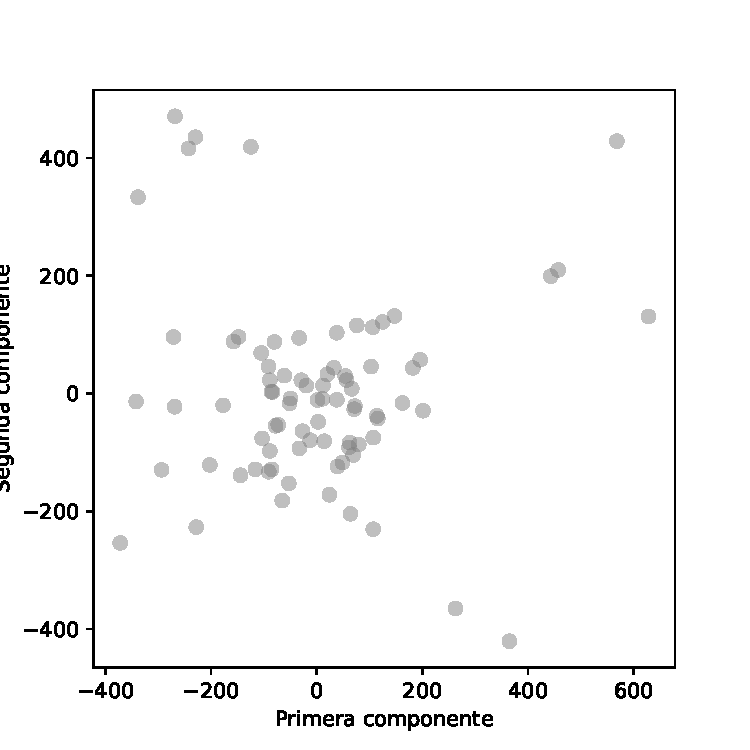
\includegraphics[width=\textwidth]{figures/pca-all-sessions-trayectory.pdf}
    \caption{}
    \label{fig:treat-pca}
  \end{subfigure}
  \begin{subfigure}{0.45\textwidth}
    \centering
    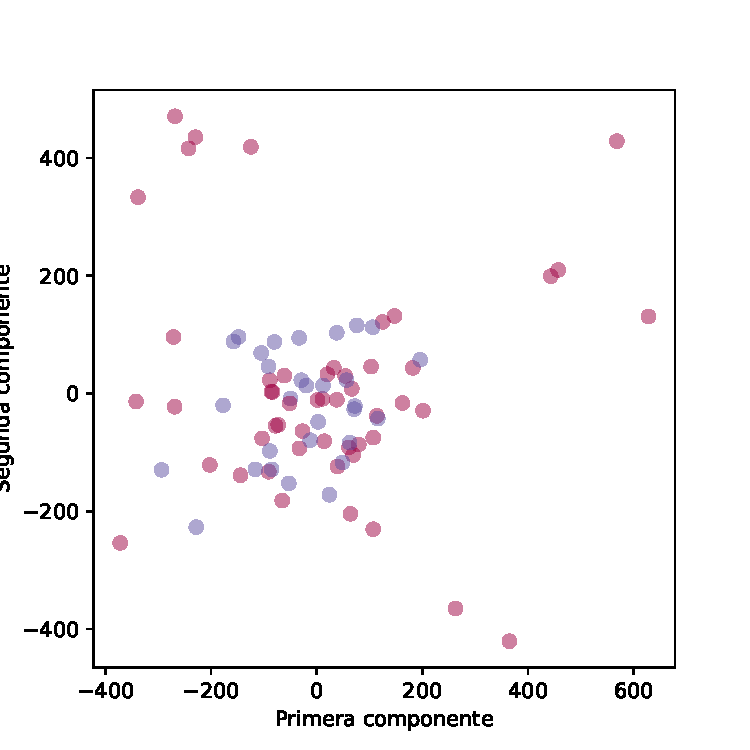
\includegraphics[width=\textwidth]{figures/true_asg-all-sessions-trayectory.pdf}
    \caption{}
    \label{fig:treat-true}
  \end{subfigure}
  \begin{subfigure}{0.45\textwidth}
    \centering
    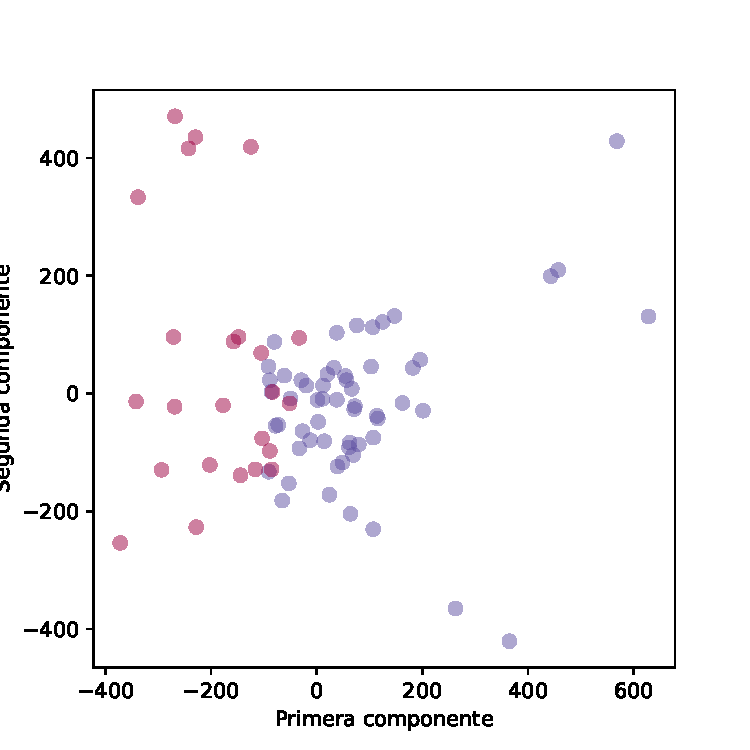
\includegraphics[width=\textwidth]{figures/kmeans_asg-all-sessions-trayectory.pdf}
    \caption{}
    \label{fig:treat-kmean}
  \end{subfigure}
  \begin{subfigure}{0.45\textwidth}
    \centering
    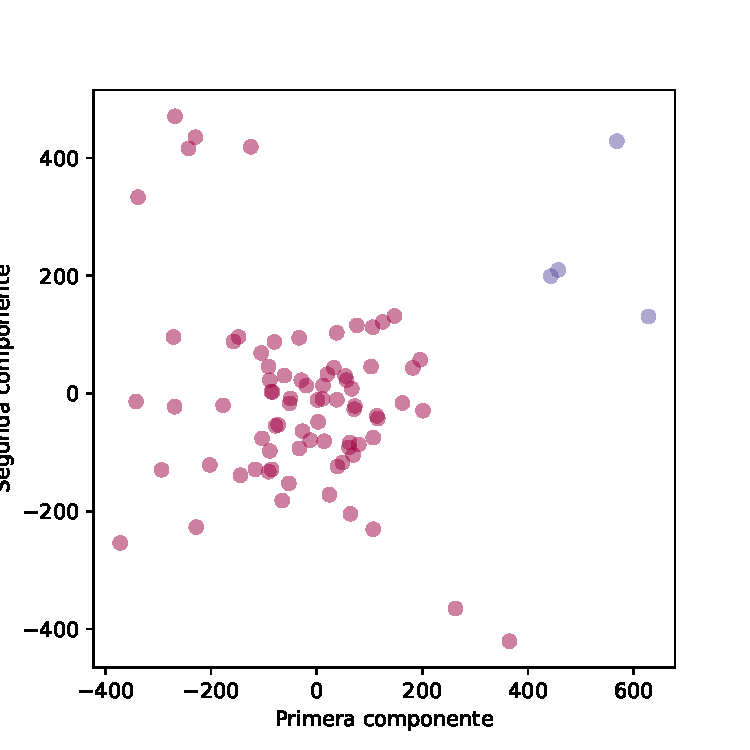
\includegraphics[width=\textwidth]{figures/agg_asg-all-sessions-trayectory.pdf}
    \caption{}
    \label{fig:treat-agg}
  \end{subfigure}
  \caption[Clasificación no supervisada de tratamiento.]{Clasificaciones no supervisadas del tipo de tratamiento. \ref{fig:treat-pca}: Distribución de los puntos de un PCA realizado sobre los datos de las 81 sesiones preprocesados y normalizados. Cada punto tiene una dimensión original de 6000 fotogramas por 52 coordenadas por fotograma, que se han linealizado para tener 312000 dimensiones por punto antes de realizar el PCA. \ref{fig:treat-true}: Asignación real del estado de cada tratamiento para cada sesión. En azul se han marcado las sesiones bajo el efecto de anticuerpos de NMDA y en rosa se han marcado las sesiones en las que no hay efecto, o se ha suministrado un tratamiento placebo. \ref{fig:treat-kmean}: Resultados de una agrupación mediante un algoritmo de k-medias sobre los puntos de las 81 sesiones con todas las dimensiones, mostrado sobre los puntos obtenidos mediante el PCA. Clases agrupadas con una precisión del $ 51,85\% $. \ref{fig:treat-agg} Resultados de una agrupación mediante un algoritmo de agrupación aglomerada sobre los puntos de las 81 sesiones con todas las dimensiones, mostrado sobre los puntos obtenidos mediante el PCA. Clases agrupadas con una precisión del $ 58,02\% $.}
  \label{fig:unsupervied-treatment}
\end{figure}


%\subsection{Agrupaciones incluyendo más variables computadas.}
%(Mismo proceso que en la sección anterior pero ahora incluyendo más variables además de la trayectoria, como velocidades, aceleración, ángulos...)

\newpage
\subsection{Agrupaciones supervisadas.}

Para aproximar una función que relaccióne 

\begin{mypython}[float={h}, caption=Red secuencial]
model = nn.Sequential(
          nn.Linear(52*1200, 1024),
          nn.Tanh(),
          nn.Linear(1024, 512),
          nn.Tanh(),
          nn.Linear(512, 128),
          nn.Tanh(),
          nn.Linear(128, 2)).to(device=device)
\end{mypython}

\begin{mypython}[float={h}, caption=Red convolucional]
class TimeSeriesNet(nn.Module):
  def __init__(self):
      super().__init__()
      self.conv1 = nn.Conv1d(in_channels=52, out_channels=104, kernel_size=3, padding=1)
      self.conv2 = nn.Conv1d(in_channels=104, out_channels=8, kernel_size=3, padding=1)
      self.fc1 = nn.Linear(2400, 32)
      self.fc2 = nn.Linear(32, 2)

  def forward(self, x):
      # Input shape: (batch_size, channels, sequence_length)
      # Max pooling with kernel size 2
      out = F.max_pool1d(torch.tanh(self.conv1(x)), 2)  
      # Max pooling with kernel size 2
      out = F.max_pool1d(torch.tanh(self.conv2(out)), 2)
      # Reshape for fully connected layer
      out = out.view(-1, 2400)  
      out = F.tanh(self.fc1(out))
      out = self.fc2(out)
      return out

model = TimeSeriesNet()
\end{mypython}